\documentclass[12pt]{article}
\title{}
\author{}
\date{}
\usepackage[margin=0.5in]{geometry}
\usepackage{graphicx,enumitem}
\begin{document}
\thispagestyle{empty}
\begin{figure}[h]\centering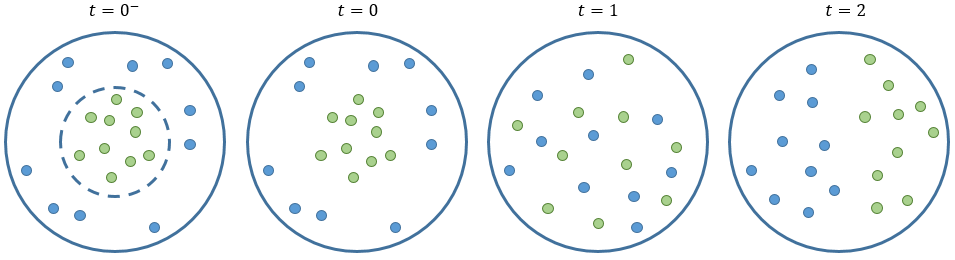
\includegraphics[width=0.6\textwidth]{Graphics/entropy_spheres.PNG}\end{figure}
Consider the system above. There are 10 molecules of $a$ and 9 molecules of $b$, each initially occupying equal volumes of a cylinder of unit depth into the page. At time 0 the partition between them is removed and the particles are allowed to mix.
\begin{enumerate}[label=(\roman*)]
\item Find the change in entropy between time $0^-$ and time 1
\item Find the change in entropy between time 1 and time 2
\item Answer (i) and (ii) if, instead of molecules, there are 10 \emph{moles} of $a$ and 9 \emph{moles} of $b$
\end{enumerate}

\begin{figure}[h]\centering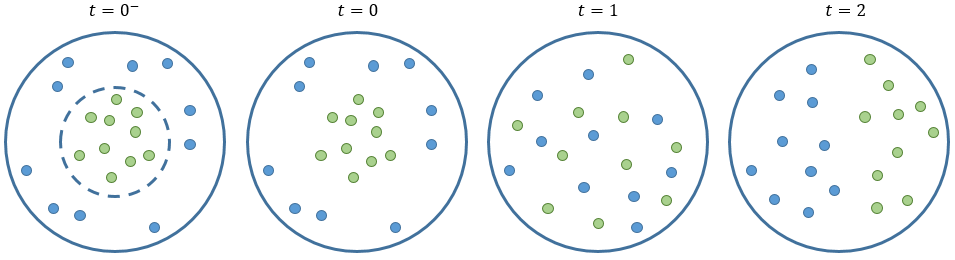
\includegraphics[width=0.6\textwidth]{Graphics/entropy_spheres.PNG}\end{figure}
Consider the system above. There are 10 molecules of $a$ and 9 molecules of $b$, each initially occupying equal volumes of a cylinder of unit depth into the page. At time 0 the partition between them is removed and the particles are allowed to mix.
\begin{enumerate}[label=(\roman*)]
\item Find the change in entropy between time $0^-$ and time 1
\item Find the change in entropy between time 1 and time 2
\item Answer (i) and (ii) if, instead of molecules, there are 10 \emph{moles} of $a$ and 9 \emph{moles} of $b$
\end{enumerate}

\begin{figure}[h]\centering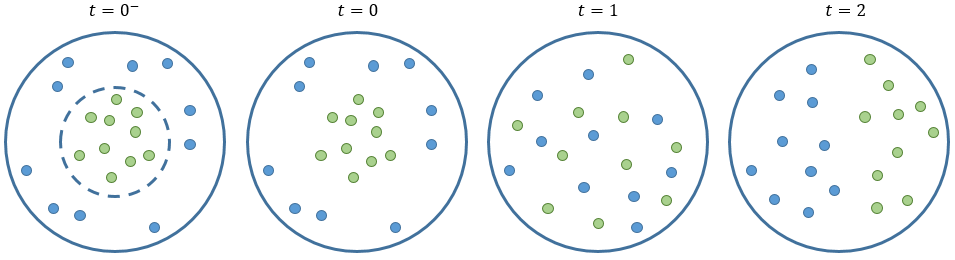
\includegraphics[width=0.6\textwidth]{Graphics/entropy_spheres.PNG}\end{figure}
Consider the system above. There are 10 molecules of $a$ and 9 molecules of $b$, each initially occupying equal volumes of a cylinder of unit depth into the page. At time 0 the partition between them is removed and the particles are allowed to mix.
\begin{enumerate}[label=(\roman*)]
\item Find the change in entropy between time $0^-$ and time 1
\item Find the change in entropy between time 1 and time 2
\item Answer (i) and (ii) if, instead of molecules, there are 10 \emph{moles} of $a$ and 9 \emph{moles} of $b$
\end{enumerate}
\end{document}